%%%%%%%%%%%%%%%%%%%%%%%%%%%%%%%%%%%%%%%%%
% Lachaise Assignment
% LaTeX Template
% Version 1.0 (26/6/2018)
%
% This template originates from:
% http://www.LaTeXTemplates.com
%
% Authors:
% Marion Lachaise & François Févotte
% Vel (vel@LaTeXTemplates.com)
%
% License:
% CC BY-NC-SA 3.0 (http://creativecommons.org/licenses/by-nc-sa/3.0/)
% 
%%%%%%%%%%%%%%%%%%%%%%%%%%%%%%%%%%%%%%%%%

%----------------------------------------------------------------------------------------
%	PACKAGES AND OTHER DOCUMENT CONFIGURATIONS
%----------------------------------------------------------------------------------------

\documentclass{article}

%%%%%%%%%%%%%%%%%%%%%%%%%%%%%%%%%%%%%%%%%
% Lachaise Assignment
% Structure Specification File
% Version 1.0 (26/6/2018)
%
% This template originates from:
% http://www.LaTeXTemplates.com
%
% Authors:
% Marion Lachaise & François Févotte
% Vel (vel@LaTeXTemplates.com)
%
% License:
% CC BY-NC-SA 3.0 (http://creativecommons.org/licenses/by-nc-sa/3.0/)
% 
%%%%%%%%%%%%%%%%%%%%%%%%%%%%%%%%%%%%%%%%%

%----------------------------------------------------------------------------------------
%	PACKAGES AND OTHER DOCUMENT CONFIGURATIONS
%----------------------------------------------------------------------------------------
\usepackage{float}
\usepackage{xcolor}
\usepackage{amsmath,amsfonts,stmaryrd,amssymb} % Math packages

\usepackage{enumerate} % Custom item numbers for enumerations
\usepackage{hyperref}
\usepackage[ruled]{algorithm2e} % Algorithms

\usepackage[framemethod=tikz]{mdframed} % Allows defining custom boxed/framed environments

\usepackage{listings} % File listings, with syntax highlighting
\lstset{
	basicstyle=\ttfamily, % Typeset listings in monospace font
}

%----------------------------------------------------------------------------------------
%	DOCUMENT MARGINS
%----------------------------------------------------------------------------------------

\usepackage{geometry} % Required for adjusting page dimensions and margins

\geometry{
	paper=a4paper, % Paper size, change to letterpaper for US letter size
	top=2.5cm, % Top margin
	bottom=3cm, % Bottom margin
	left=2.5cm, % Left margin
	right=2.5cm, % Right margin
	headheight=14pt, % Header height
	footskip=1.5cm, % Space from the bottom margin to the baseline of the footer
	headsep=1.2cm, % Space from the top margin to the baseline of the header
	%showframe, % Uncomment to show how the type block is set on the page
}

%----------------------------------------------------------------------------------------
%	FONTS
%----------------------------------------------------------------------------------------

\usepackage[utf8]{inputenc} % Required for inputting international characters
\usepackage[T1]{fontenc} % Output font encoding for international characters

\usepackage{XCharter} % Use the XCharter fonts

%----------------------------------------------------------------------------------------
%	COMMAND LINE ENVIRONMENT
%----------------------------------------------------------------------------------------

% Usage:
% \begin{commandline}
%	\begin{verbatim}
%		$ ls
%		
%		Applications	Desktop	...
%	\end{verbatim}
% \end{commandline}

\mdfdefinestyle{commandline}{
	leftmargin=10pt,
	rightmargin=10pt,
	innerleftmargin=15pt,
	middlelinecolor=black!50!white,
	middlelinewidth=2pt,
	frametitlerule=false,
	backgroundcolor=black!5!white,
	frametitle={Command Line},
	frametitlefont={\normalfont\sffamily\color{white}\hspace{-1em}},
	frametitlebackgroundcolor=black!50!white,
	nobreak,
}

% Define a custom environment for command-line snapshots
\newenvironment{commandline}{
	\medskip
	\begin{mdframed}[style=commandline]
}{
	\end{mdframed}
	\medskip
}

%----------------------------------------------------------------------------------------
%	FILE CONTENTS ENVIRONMENT
%----------------------------------------------------------------------------------------

% Usage:
% \begin{file}[optional filename, defaults to "File"]
%	File contents, for example, with a listings environment
% \end{file}

\mdfdefinestyle{file}{
	innertopmargin=1.6\baselineskip,
	innerbottommargin=0.8\baselineskip,
	topline=false, bottomline=false,
	leftline=false, rightline=false,
	leftmargin=2cm,
	rightmargin=2cm,
	singleextra={%
		\draw[fill=black!10!white](P)++(0,-1.2em)rectangle(P-|O);
		\node[anchor=north west]
		at(P-|O){\ttfamily\mdfilename};
		%
		\def\l{3em}
		\draw(O-|P)++(-\l,0)--++(\l,\l)--(P)--(P-|O)--(O)--cycle;
		\draw(O-|P)++(-\l,0)--++(0,\l)--++(\l,0);
	},
	nobreak,
}

% Define a custom environment for file contents
\newenvironment{file}[1][File]{ % Set the default filename to "File"
	\medskip
	\newcommand{\mdfilename}{#1}
	\begin{mdframed}[style=file]
}{
	\end{mdframed}
	\medskip
}

%----------------------------------------------------------------------------------------
%	NUMBERED QUESTIONS ENVIRONMENT
%----------------------------------------------------------------------------------------

% Usage:
% \begin{question}[optional title]
%	Question contents
% \end{question}

\mdfdefinestyle{question}{
	innertopmargin=1.2\baselineskip,
	innerbottommargin=0.8\baselineskip,
	roundcorner=5pt,
	nobreak,
	singleextra={%
		\draw(P-|O)node[xshift=1em,anchor=west,fill=white,draw,rounded corners=5pt]{%
		Question \theQuestion\questionTitle};
	},
}

\newcounter{Question} % Stores the current question number that gets iterated with each new question

% Define a custom environment for numbered questions
\newenvironment{question}[1][\unskip]{
	\bigskip
	\stepcounter{Question}
	\newcommand{\questionTitle}{~#1}
	\begin{mdframed}[style=question]
}{
	\end{mdframed}
	\medskip
}

%----------------------------------------------------------------------------------------
%	WARNING TEXT ENVIRONMENT
%----------------------------------------------------------------------------------------

% Usage:
% \begin{warn}[optional title, defaults to "Warning:"]
%	Contents
% \end{warn}

\mdfdefinestyle{warning}{
	topline=false, bottomline=false,
	leftline=false, rightline=false,
	nobreak,
	singleextra={%
		\draw(P-|O)++(-0.5em,0)node(tmp1){};
		\draw(P-|O)++(0.5em,0)node(tmp2){};
		\fill[black,rotate around={45:(P-|O)}](tmp1)rectangle(tmp2);
		\node at(P-|O){\color{white}\scriptsize\bf !};
		\draw[very thick](P-|O)++(0,-1em)--(O);%--(O-|P);
	}
}

% Define a custom environment for warning text
\newenvironment{warn}[1][Warning:]{ % Set the default warning to "Warning:"
	\medskip
	\begin{mdframed}[style=warning]
		\noindent{\textbf{#1}}
}{
	\end{mdframed}
}

%----------------------------------------------------------------------------------------
%	INFORMATION ENVIRONMENT
%----------------------------------------------------------------------------------------

% Usage:
% \begin{info}[optional title, defaults to "Info:"]
% 	contents
% 	\end{info}

\mdfdefinestyle{info}{%
	topline=false, bottomline=false,
	leftline=false, rightline=false,
	nobreak,
	singleextra={%
		\fill[black](P-|O)circle[radius=0.4em];
		\node at(P-|O){\color{white}\scriptsize\bf i};
		\draw[very thick](P-|O)++(0,-0.8em)--(O);%--(O-|P);
	}
}

% Define a custom environment for information
\newenvironment{info}[1][Info:]{ % Set the default title to "Info:"
	\medskip
	\begin{mdframed}[style=info]
		\noindent{\textbf{#1}}
}{
	\end{mdframed}
}
 % Include the file specifying the document structure and custom commands

%----------------------------------------------------------------------------------------
%	ASSIGNMENT INFORMATION
%----------------------------------------------------------------------------------------

\title{MMOD101: Workshop ``Visualizing 3D structures with Pymol''} % Title of the assignment

\author{Alexey K. Shaytan\\ \texttt{alex@intbio.org}} % Author name and email address

\date{Lomonosov Moscow State University --- \today} % University, school and/or department name(s) and a date

%----------------------------------------------------------------------------------------

\begin{document}

\maketitle % Print the title

%----------------------------------------------------------------------------------------
%	INTRODUCTION
%----------------------------------------------------------------------------------------
\begin{warn}[Requirements:]

Pymol \url{http://www.pymol.org} 

3-button mouse
\end{warn}


    PyMOL is a molecular modeling software used for making publication-quality renders of biochemical structures. Using PyMOL, it is possible to make high quality images, analyze and manipulate structures.


\begin{figure}[h!]
    \centering
    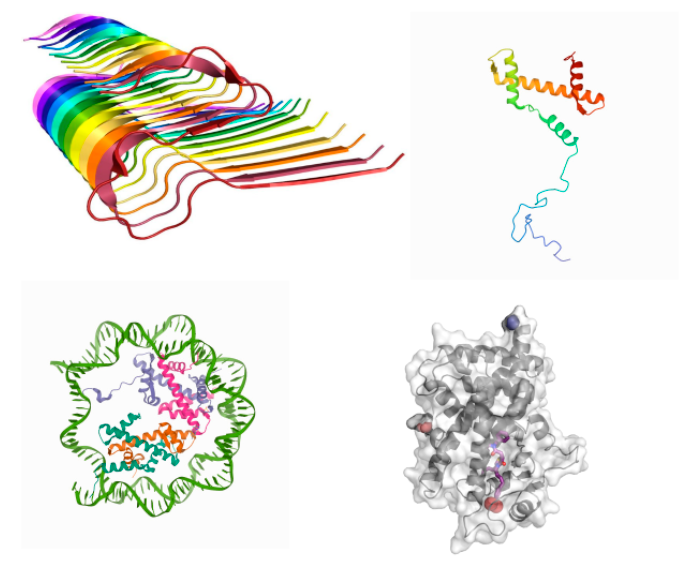
\includegraphics[width=0.5\textwidth]{workshops/pymol/imgs/intrimg1.png}
    \caption[]{Example of structure visualization}
    \label{intfig1}
\end{figure}

\tableofcontents

%Pymol user interface orientation
% Download and open PDB structure
% Making selections in PDB structures and visualizing them.
% Pymol selection language
% Rotating, translating, setting clipping planes, projection type, etc.
% Different representations: bonds, CPK, VdW.
% Molecular surfaces
% Structure alignment
% Adding H-atoms.
% Morphing, visualizing conformational transitions.
% Coloring structure by parameters (B-factors)
% Comparing PDB with electron density.
% Python scripting

\section{User interface orientation}

\textbf{Below is the PyMOL window:}



%paste interface image
\begin{figure}[H]
    \centering
    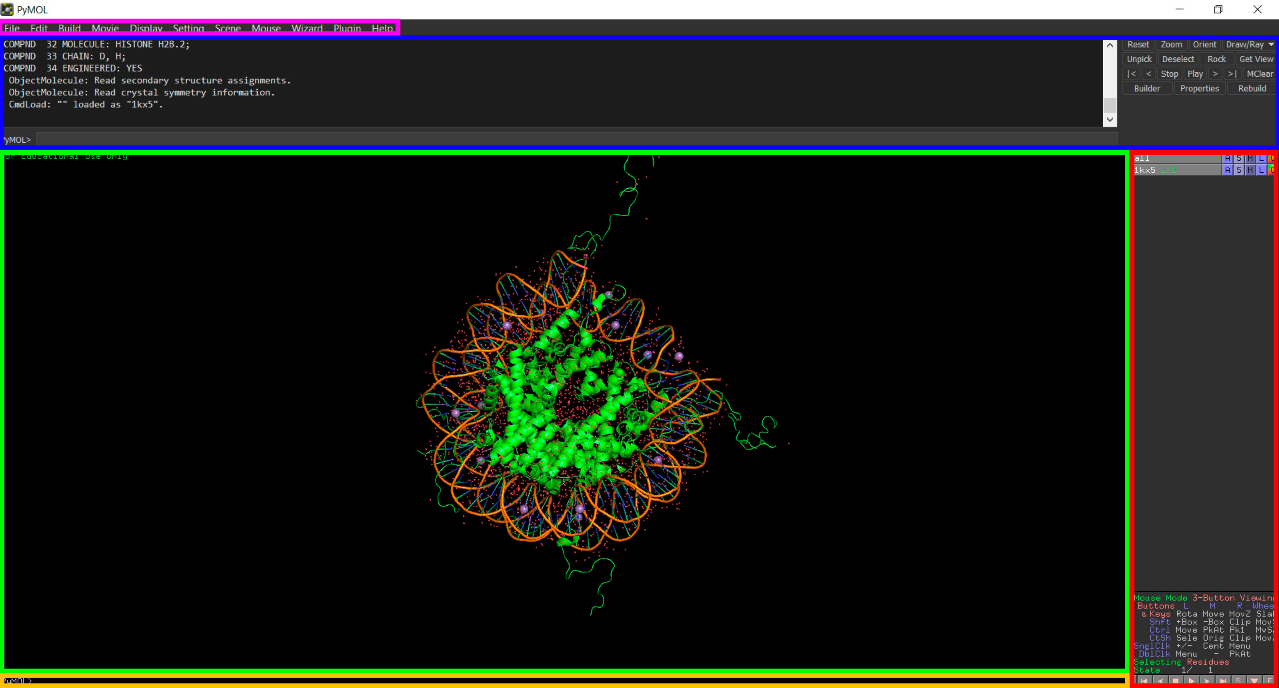
\includegraphics[width=1.0\textwidth]{workshops/pymol/imgs/interfaceimage.png}
    \caption[]{User interface}
    \label{interfaceimg}
\end{figure}

\begin{itemize}
    \item {\color{blue} \textbf{``Upper Control Panel''}} - you can work with commands (open file, color ``selection'', etc.)
    
    \item {\color{orange} \textbf{``Command line''}} - this line mostfully use pro users, in this course we won't work with that line \\
    
    \item  {\color{red} \textbf{``Object Control Panel, Mouse Control Legend''}} - here you can work with objects, change mouse control and work with scene control buttons. \\

    \item {\color{purple} \textbf{``Toolbar''}} - on this bar we have usefull tools for work.

    \item {\color{green} \textbf{``Display area''}} - try to play with the mouse controls.
   
\end{itemize}





\section{Download and open PDB structure}

In Toolbar click \textbf{File} and select \textbf{Get PDB}, then a dilog window will open:\\

Write \textbf{1kx5} \\

Click \textbf{Download} and the selected structure will load. \\

%paste dilog window image
\begin{figure}[H]
    \centering
    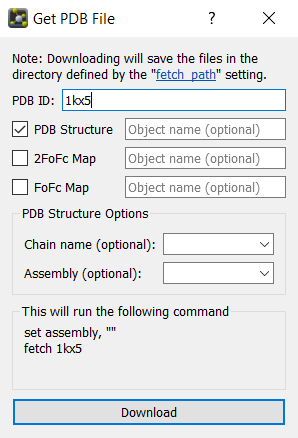
\includegraphics[width=0.3\textwidth]{workshops/pymol/imgs/dialogwindow.png}
    \caption[]{Dialog window}
    \label{dialogwindow}
\end{figure}

Also if we downloaded file structure from internet, we can open it from our desktop, as we see i have this file type \textbf{.pdb} on my desktop that called 1kx5: \\

%image file
\begin{figure}[H]
    \centering
    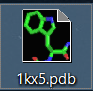
\includegraphics[width=0.1\textwidth]{workshops/pymol/imgs/dtfileimg.png}
    \caption[]{Desktop file}
    \label{dtfile}
\end{figure}

We can open it by double clicking on it or we'll go to \textbf{Upper Control Panel} and write this command: (\textbf{fetch 1kx5}) \\

%paste image of upper control panel command
\begin{figure}[H]
    \centering
    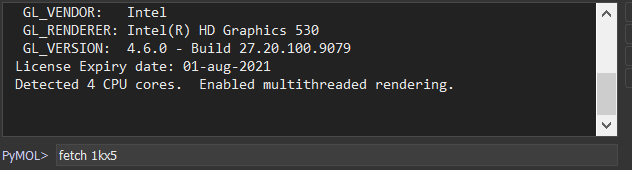
\includegraphics[width=0.6\textwidth]{workshops/pymol/imgs/ucpcmd.png}
    \caption[]{}
    \label{ucpcommand}
\end{figure}

Then press \textbf{Enter} and strusture will open \\

%paste image view
\begin{figure}[H]
    \centering
    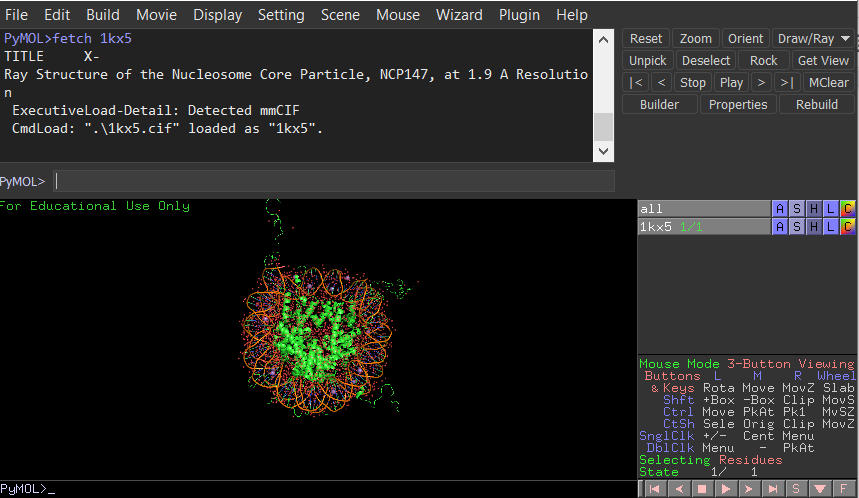
\includegraphics[width=0.7\textwidth]{workshops/pymol/imgs/imgview1.png}
    \caption[]{}
    \label{view1}
\end{figure}

\begin{center}
    \textbf{Basic mouse control:}
\end{center}

\begin{itemize}
\item \textbf{Left click:} rotates the model, click in the center allows free control. As you drag around the edges, it will rotate around the Z axis.

\item \textbf{Right Click:} zoom and out structure.

\item \textbf{Middle Mouse Button:} when you click on a squirrel, it moves around the preview window without rotating.

\end{itemize}





\section{Rotating, translating, setting clipping planes, projection type, centering (actions) etc.}

\begin{itemize}

    \item \textbf{Rotating:} press \textbf{Right mouse button} and move mouse.

    \item \textbf{Translating:} ...

    \item \textbf{Setting clipping planes:} you can scrool mouse wheel to move clipping planes

    \item \textbf{Projection type:} in \textbf{Toolbar} click on \textbf{Display} and select \textbf{Orthoscopic View}

    \item \textbf{Centering:} Press \textbf{Action} button and select \textbf{center}. The structure will rotate around ``center point''. Also you can select \textbf{orient}, it will rotate structure in comfortable, front view.

\textbf{CTRL+ Left Click:} will center veiw on object you click

    \item \textbf{Double Left Click on structure lement:} will open quick tool menu of structure

\end{itemize}





\section{Structure visualization modes (presets, lines, sticks, spheres)}
\begin{itemize}

    \item \textbf{Presets:} press \textbf{Action} button near structure name block, in \textbf{Preset} section and click on \textbf{Publication} you have chosen one of several types of projection.
    
    \item \textbf{Lines/sticks/spheres:} press \textbf{Show} button, aim on \textbf{as} and select \textbf{lines/sticks/spheres}
    
\end{itemize}





\section{Making selections (by chains, sequence, etc.).}

To make chain selection you need to Double click left mouse button on element you want to select, then aim on ``chain'' and select ``sele''

\textbf{Sequence selection:} in right bottom angle you can see \textbf{Scene Control Panel}, press {\color{pink} {\Large \textbf{S}}} panel button opens the protein sequence, than you can select section you need.

\begin{figure}[h!]
    \centering
    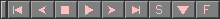
\includegraphics[width=0.5\textwidth]{workshops/pymol/imgs/panel.png}
    \caption[]{Scene Control Panel}
    \label{panel}
\end{figure}







\section{Pymol selection language}

Try to use this command:

>show spheres, solvent and chain A

To make structure look default write:

> as cartoon

List of commands you can see on this \href{https://pymolwiki.org/index.php/Selection_Algebra}{site}








\section{Molecular surfaces}

Press {\Large \textbf{S}}(Show) button, then aim on \textbf{as} and select surface

Also you can write command: 

>as surface







\section{Structure alignment}

For alignment to write command, or in Toolbar select \textbf{Plugin>Align} in opened window choose structures and press OK

Here is a command > align structure1, structure2

If i have these strustures
1) 1kx5
2) 1kt4

I'll write > align 1kx5, 1kt4






\section{Manipulating, moving structure (actions)}

If you have a certain amount of structures, and you want to move them relative to each other, follow this steps:

\begin{itemize}

    \item[1)] Look at \textbf{Mouse Control Legend} and press on {\color{green} \textbf{Mose Mode}}, it must change to {\color{pink} 3- Butoon Editing}
    
    \item[2)] To rotate structure relative to each other press \textbf{Shift + Left Mouse Button}, to move it press \textbf{Shift + Middle Mouse Button}
    
    \item[3)] Also you can bend elements of your structure, press on element you want to bend \textbf{CTRL + Left Mouse Button}
    
\end{itemize}








\section{Adding H-atoms.}

To add Hydrogen atoms, you must use command >h\_add (name of sele, structure)








\section{Calculating charge}

Press {\Large \textbf{A}}(Action) button, \textbf{Compute>Charges>formal charge sum}








\section{Morphing, visualizing conformational transitions.}

To morph structures, press {\Large \textbf{A}}(Action) button, \textbf{Generate>Morph>to molecule(choose the molecule)}








\section{Coloring structure by parameters (B-factors)}

spectrum b, blue\_red, minimum=10, maximum=50

spectrum count, rainbow\_rev, chain A, byres=1







\section{Comparing PDB with electron density.}

Go to \textbf{Plugin > APBS Electrostatics} in opened window press \textbf{Run}


\begin{figure}[H]
    \centering 
    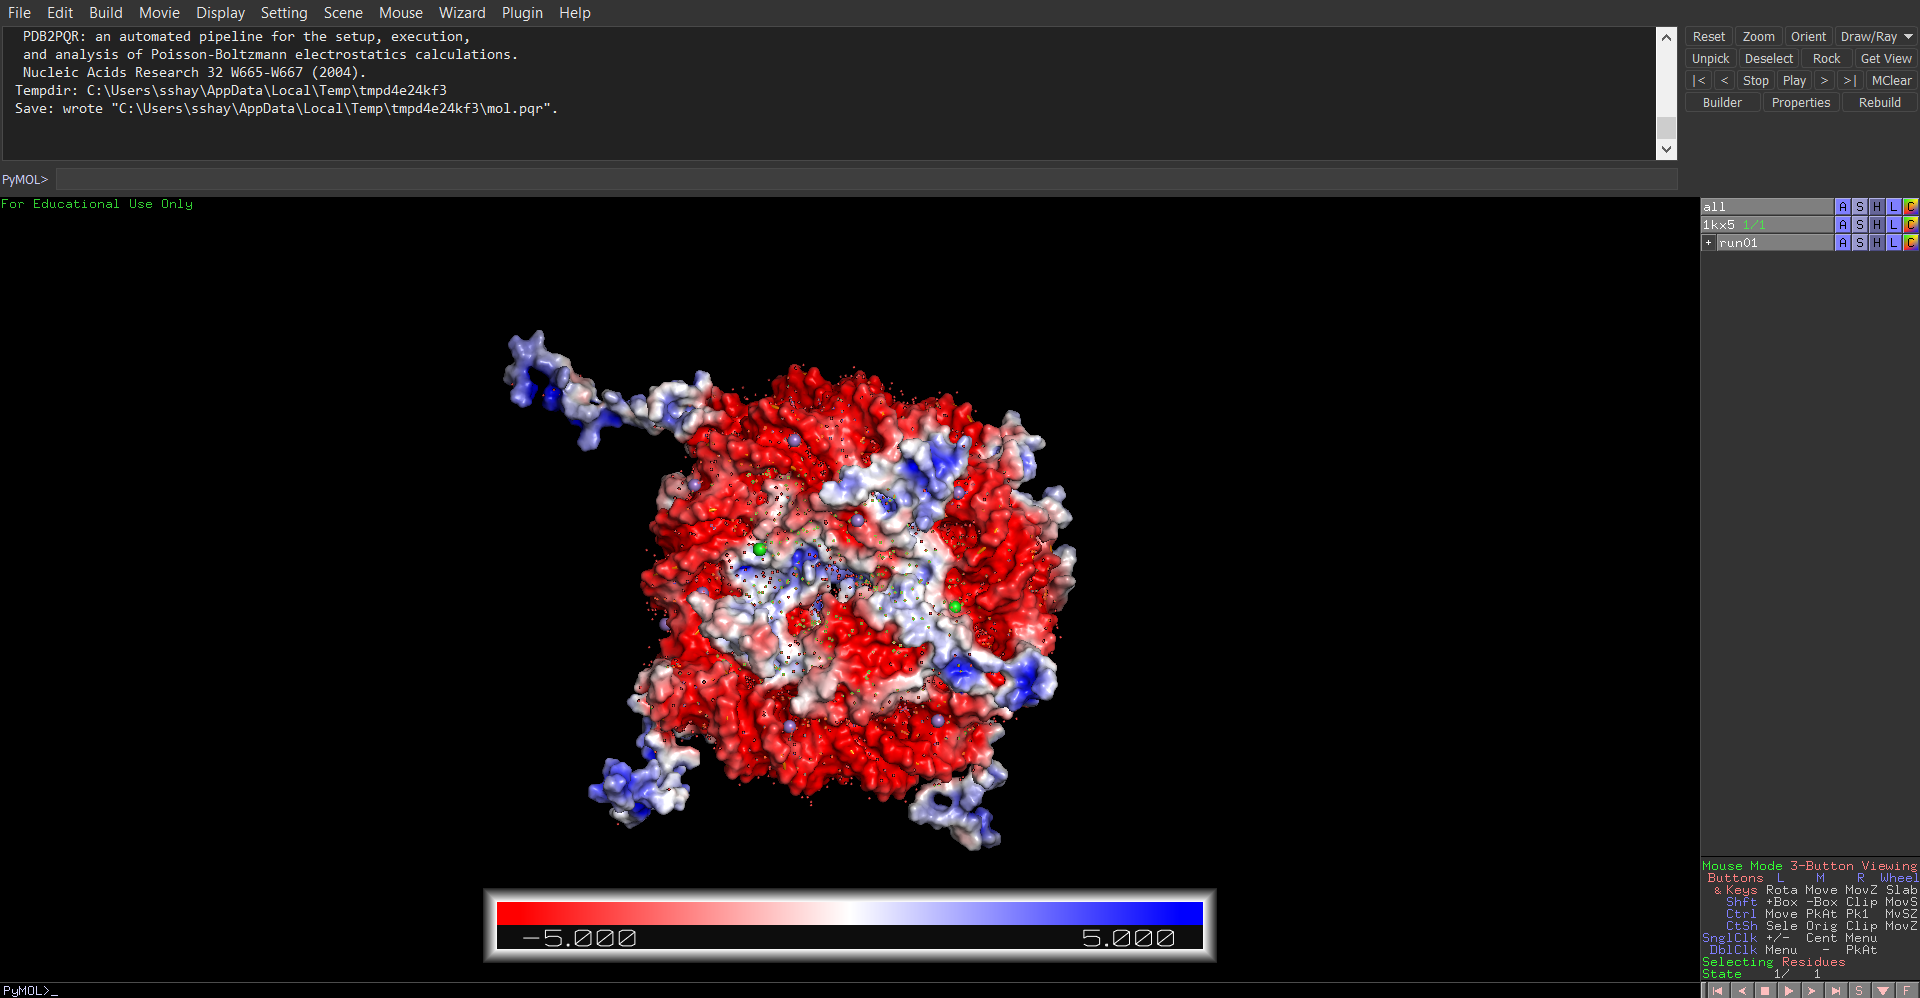
\includegraphics[width=1\textwidth]{workshops/pymol/imgs/1kx5 Elcetrostatics.png}
    \caption{APBS Electrostatics}
    \label{fig:my_label}
\end{figure}








\section{Scripting}
In PyMOL scripts are wery useful tool. Script in PyMOL - is a file with list of commands, that helps you to save time.

Some of them you can look on this \href{https://pymolwiki.org/index.php/Running_Scripts}{site}








\section{Object control panel}

If you look to the right of the \textbf{Display area}, you will notice an area with different \textbf{blocks} including the PDB name "1kx5". This is called the back-end GUI: \\


%paste feild image
\begin{figure}[h!]
    \centering
    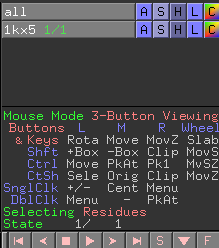
\includegraphics[width=0.3\textwidth]{workshops/pymol/imgs/field.png}
    \caption[]{}
    \label{field}
\end{figure}


\textbf{Blocks -} \\  
%paste blocks image
\begin{figure}[h!]
    \centering
    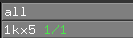
\includegraphics[width=0.3\textwidth]{workshops/pymol/imgs/blocks.png}
    \caption[]{Blocks}
    \label{blocks}
\end{figure}




You can hide elements from your \textbf{Display area} by clicking on the \textbf{block} with their name. \\

Let's pay attention to these buttons: \\

%paste bottons image
\begin{figure}[h!]
    \centering
    
\includegraphics[width=0.3\textwidth]{workshops/pymol/imgs/buttons.png}
    \caption[]{Buttons}
    \label{buttons}
\end{figure}

Each of these letters corresponds to an option for visualization:

\textbf{A: Action}, allows the user to orient the camera and move the protein around, edit the structure.

\textbf{S: Show}, will show a representation type of the visual, such as cartoon, spheres, sticks.

\textbf{H: Hide}, will hide a representation type of the visual.

\textbf{L: Label}, allows the labelling of different aspects of the visual.

\textbf{C: Color}, will color the visual based on the user selection. \\

Let's also pay attention to this panel located in the lower right corner. \\

%paste panel image
\begin{figure}[h!]
    \centering
    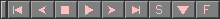
\includegraphics[width=0.5\textwidth]{workshops/pymol/imgs/panel.png}
    \caption[]{Scene Control Panel}
    \label{panel}
\end{figure}

The {\color{pink} {\Large \textbf{S}}} panel button opens the protein sequence, it will be displayed at the top of \textbf{Display panel}.

%paste sequence image
\begin{figure}[h!]
    \centering
    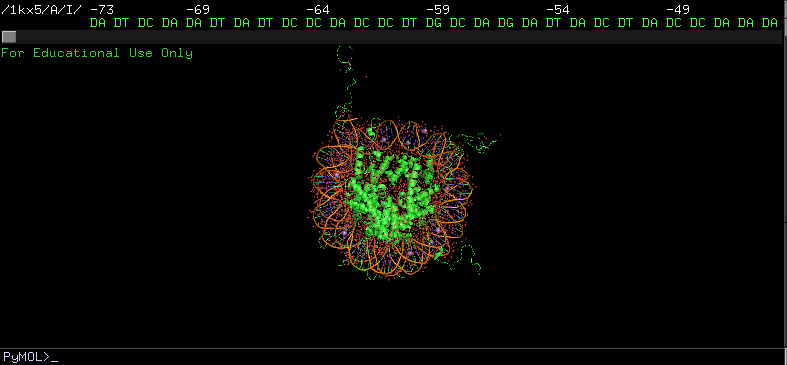
\includegraphics[width=0.7\textwidth]{workshops/pymol/imgs/sequense.png}
    \caption[]{}
    \label{sequence}
\end{figure}

The sequence can also be selected and colored.

In this image, we have selected 21 atoms, this can be seen in the \textbf{Upper Control Panel}, we can observe that on our structure the selected segment of the sequence is displayed as pink squares. \\

%paste sequense selection image
\begin{figure}[h!]
    \centering
    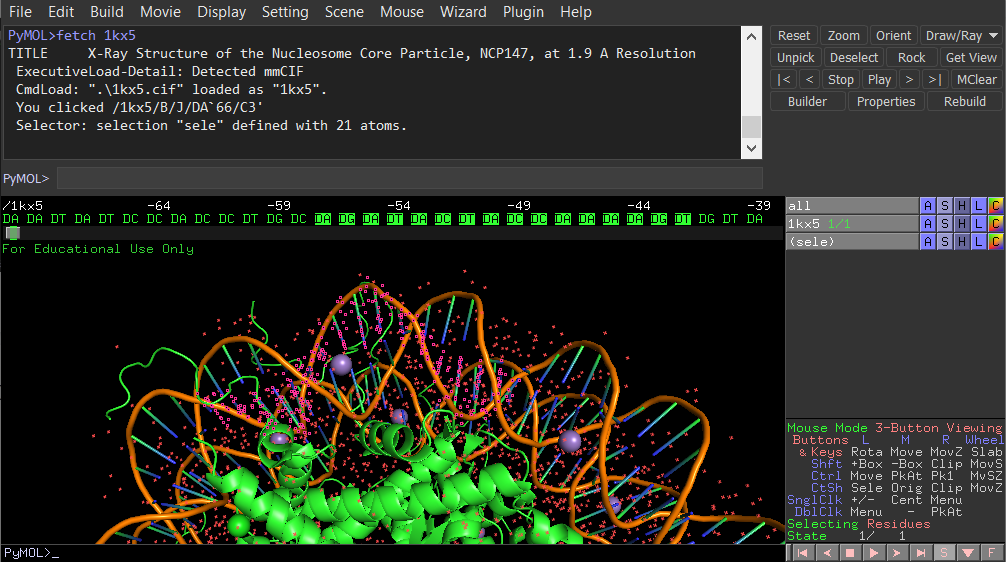
\includegraphics[width=0.7\textwidth]{workshops/pymol/imgs/sequencesele.png}
    \caption[]{}
    \label{sequencesele}
\end{figure}

Also, a new \textbf{block} called \textbf{(sele)} has appeared, with which you can further work, let's say you need to color this segment of the sequence, press {\Large \textbf{C}}
and choose the color. \\

%paste colored sequence selection image
\begin{figure}[h!]
    \centering
    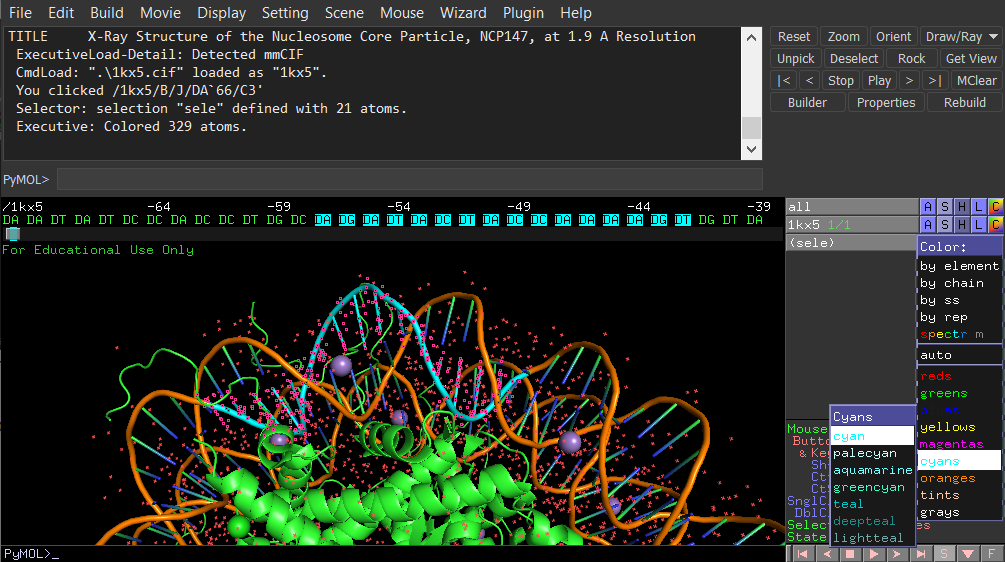
\includegraphics[width=0.7\textwidth]{workshops/pymol/imgs/sequenceseleclr.png}
    \caption[]{}
    \label{sequenceseleclr}
\end{figure}

We see how this segment is colored in the color we need.

With the help of the {\Large \textbf{H}} button we can hide the selected segment. \\

%paste hidden sequence image
\begin{figure}[h!]
    \centering
    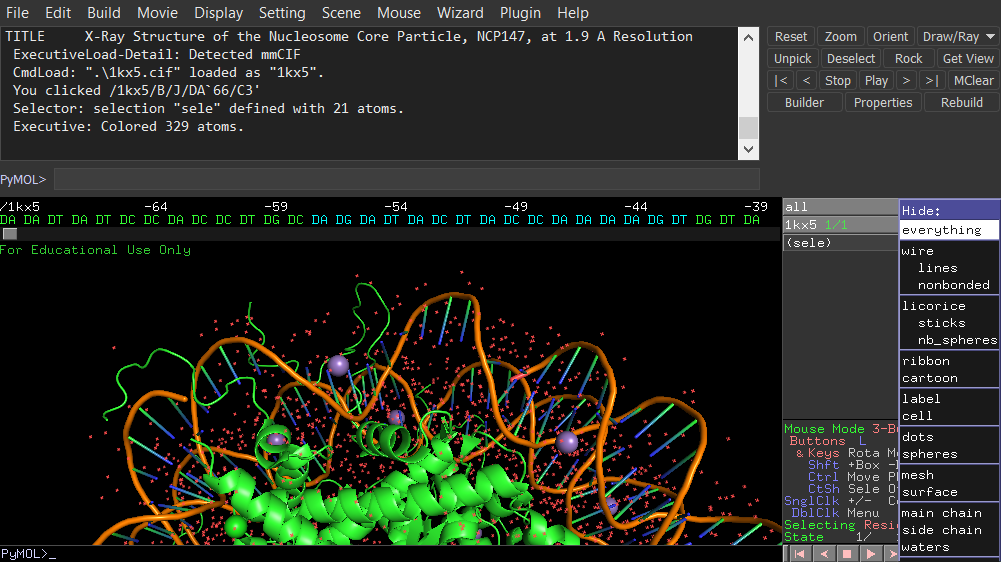
\includegraphics[width=0.7\textwidth]{workshops/pymol/imgs/hiddensequence.png}
    \caption[]{}
    \label{hiddensequence}
\end{figure}

And the selected segment disappears.

To return it, click on the button {\Large \textbf{S}} and select the \textbf{cartoon} line, below you can see that our segment is displayed back. \\


\section{Toolbar}

The interface also contains most of the tools needed to use PyMOL. We will break down each tool individually in a square corresponding to the color in the picture below. \\

%paste toolbar image
\begin{figure}[h!]
    \centering
    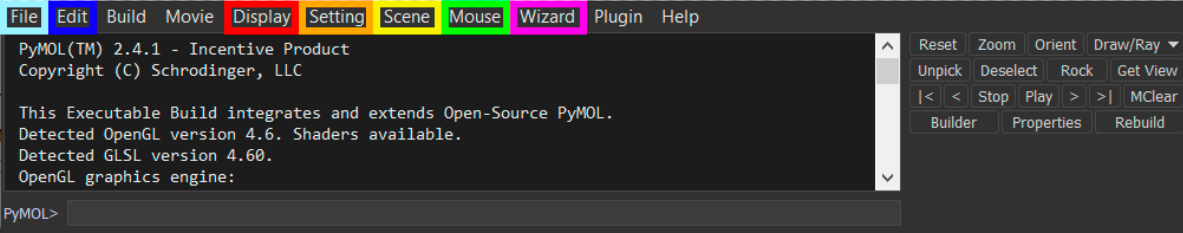
\includegraphics[width=0.9\textwidth]{workshops/pymol/imgs/toolbar.png}
    \caption[]{}
    \label{toolbar}
\end{figure}

\begin{center}
    \Large \textbf{File}
\end{center}

As with most programs, this tab is used to open, save and export files. When you click on it, the following options appear: \\

%paste FILE tab image
\begin{figure}[h!]
    \centering
    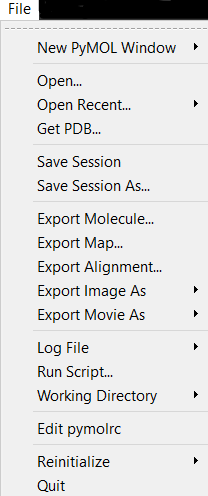
\includegraphics[width=0.3\textwidth]{workshops/pymol/imgs/filetab.png}
    \caption[]{}
    \label{filetab}
\end{figure}

\begin{itemize}
\item \textbf{“New PyMOL Window”:} Allows you to open a new window, you can have multiple open at once.

\item \textbf{“Open” and “Open Recent…”:} Opens either structures to view in PyMOL or entire PyMOL .pse sessions.

\item \textbf{“Get PDB…”:} Allows you to fetch a model of a PDB and directly import into the session.

\item \textbf{“Save Session” and “Save Session As…”:} Saves the current session as a .pse file. A .pse file is a PyMOL session file. 

\item \textbf{“Export Molecule…”:} Allows you to export a model on screen to a file format (e.g. .pdb) 

\item \textbf{“Export Image As”:} Exports the current view on screen to an image.

\item \textbf{“Export Movie As”:} Export the current movie timeline to a video file.

\item \textbf{“Reinitialize”:} Reruns all the settings and display options currently enabled.

\end{itemize}



\begin{center}
    \Large \textbf{Edit}
\end{center}

This tab allows you to redo or undo things in PyMOL \\

%paste EDIT tab image
\begin{figure}[h!]
    \centering
    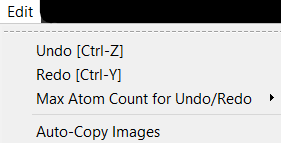
\includegraphics[width=0.4\textwidth]{workshops/pymol/imgs/edittab.png}
    \caption[]{}
    \label{edittab}
\end{figure}

\begin{itemize}
    \item \textbf{CTRL + Z} and \textbf{CTRL + Y} are shortcuts that you can use
    
    \item The maximum number of atoms can be adjusted for large images, but in most cases it is best to leave the default settings.
\end{itemize}




\begin{center}
    \Large \textbf{Display}
\end{center}

This tab houses the options that alter the display in the viewport of PyMOL \\

%paste DISPLAY tab image
\begin{figure}[h!]
    \centering
    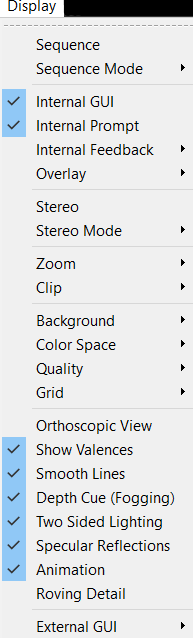
\includegraphics[width=0.3\textwidth]{workshops/pymol/imgs/displaytab.png}
    \caption[]{}
    \label{displaytab}
\end{figure}

\begin{itemize}

\item \textbf{“Sequence”:} Displays the sequence of amino acids or nucleic acids in a protein or piece of DNA above the preview 

\item \textbf{“Sequence Mode”:} Changes what the sequence displays

\item \textbf{“Background”:} Option to change the color and type of background visible

\item \textbf{“Color Space”:} Houses settings for different color spaces, can allow for different aesthetic appearances

\item \textbf{“Quality”:} Provides options for the level of quality of the visualization shown. This option is useful for less powerful computers

\item \textbf{“Grid”:} Allows the option to display objects in a grid

\item \textbf{“Orthoscopic View”:} Toggles the orthoscopic view setting, which slightly distorts the preview window to enhance depth perception

\item \textbf{“Show Valances”:}  Toggles the visibility of valences in models

\item \textbf{“Depth Cue (Fogging)”:} Toggles fog that helps with depth perception

\end{itemize}



\begin{center}
    \Large \textbf{Settings}
\end{center}

This tab holds the settings for the representations of structures on screen \\

%paste SETTING tab image
\begin{figure}[h!]
    \centering
    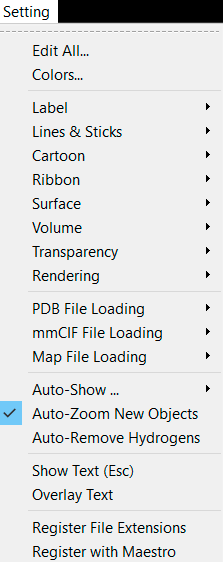
\includegraphics[width=0.3\textwidth]{workshops/pymol/imgs/settingtab.png}
    \caption[]{}
    \label{settingtab}
\end{figure}

\begin{itemize}

\item \textbf{“Edit All…”:}  This will bring up a menu of all the advanced settings available in PyMOL, this will be explored further in the advanced tutorial

\item \textbf{“Colors…”:}  Allows you to change the color of atom types, and of preset colors available in the menu (ie make all phosphorous green)

\item \textbf{“Label” →  “Transparency”:}  Allows you to tweak settings of visualization.

\item \textbf{“Auto-Zoom New Objects”:}  Will force zoom to objects as they are loaded in

\item \textbf{“Auto-Remove Hydrogens”:}  Removes hydrogens from objects as they are loaded in

\end{itemize}


\begin{center}
    \Large \textbf{Scene}
\end{center}

This allows for the storage of perspectives and visualizations as scenes that can be retrieved at a later point. This is very useful for moments when multiple representation types are necessary for a single protein. \\

%paste SCENE tab image
\begin{figure}[h!]
    \centering
    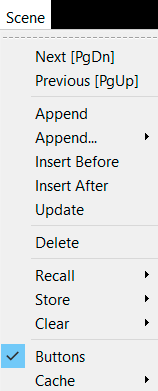
\includegraphics[width=0.2\textwidth]{workshops/pymol/imgs/scenetab.png}
    \caption[]{}
    \label{scenetab}
\end{figure}

\begin{itemize}

\item \textbf{“Next”:}  Switches to the next scene, can be called by using the [PgDn] key

\item \textbf{“Previous”:}  Switches to the previous scene, can be called by using the [PgUp] key

\item \textbf{“Append”:}  Makes a new scene from the settings currently present, automatically assigning the name as a number

\item \textbf{“Insert Before” and “Insert After”:}  Does the same as Append, but will create the scene before or after the current scene toggled on

\item \textbf{“Update”:}  Overwrites the current scene 

\item \textbf{“Delete”:}  Deletes current scene

\item \textbf{“Recall”:}  Will toggle a scene from a list of F1 to F12. Scenes can also be recalled by using the buttons at the bottom left of the screen

\item \textbf{“Store”:}  Allows you to store a scene from F1 to F12

\item \textbf{“Clear”:}  Clears a scene F1 to F12

\end{itemize}


\begin{center}
    \Large \textbf{Mouse}
\end{center}

This tab provides the options \\

%paste MOUSE tab image
\begin{figure}[h!]
    \centering
    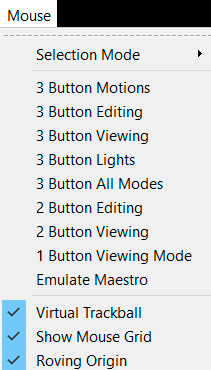
\includegraphics[width=0.2\textwidth]{workshops/pymol/imgs/mousetab.png}
    \caption[]{}
    \label{mousetab}
\end{figure}

\begin{itemize}

\item \textbf{“Selection Mode”:} Houses the different selection modes for picking parts of the model on screen

\item \textbf{“Emulate Maestro”:} Sets the mouse control settings to that of Maestro, and allows the user to select by dragging a box across the screen


\end{itemize}


\begin{center}
    \Large \textbf{Wizard}
\end{center}

This tab provides special modes that provides useful tools to measure, change appearance, etc. 
 \\

%paste WIZARD tab image
\begin{figure}[h!]
    \centering
    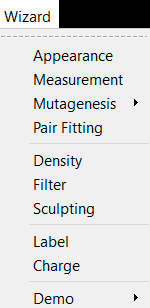
\includegraphics[width=0.2\textwidth]{workshops/pymol/imgs/wizardtab.png}
    \caption[]{}
    \label{wizardtab}
\end{figure}

\begin{itemize}

\item \textbf{“Appearance”:} Allows the user to quickly toggle through showing certain aspects of the visualization (ie quickly hide and show sticks)

\item \textbf{“Measurement”:} One of the most useful, measures the distance between two objects

\item \textbf{“Mutagenesis”:} Allows the user to mutate residues or nucleic acids by rotation, substitution, etc. 

\item \textbf{“Label”:} Can toggle the labels for certain residues of the visualization

\item \textbf{“Demo”:} Allows the user to play around with some demonstrations of what PyMOL can do, let's choose \textbf{Representation} and we'll see:

\end{itemize}

%paste REPRESENTATION IMAGE
\begin{figure}[h!]
    \centering
    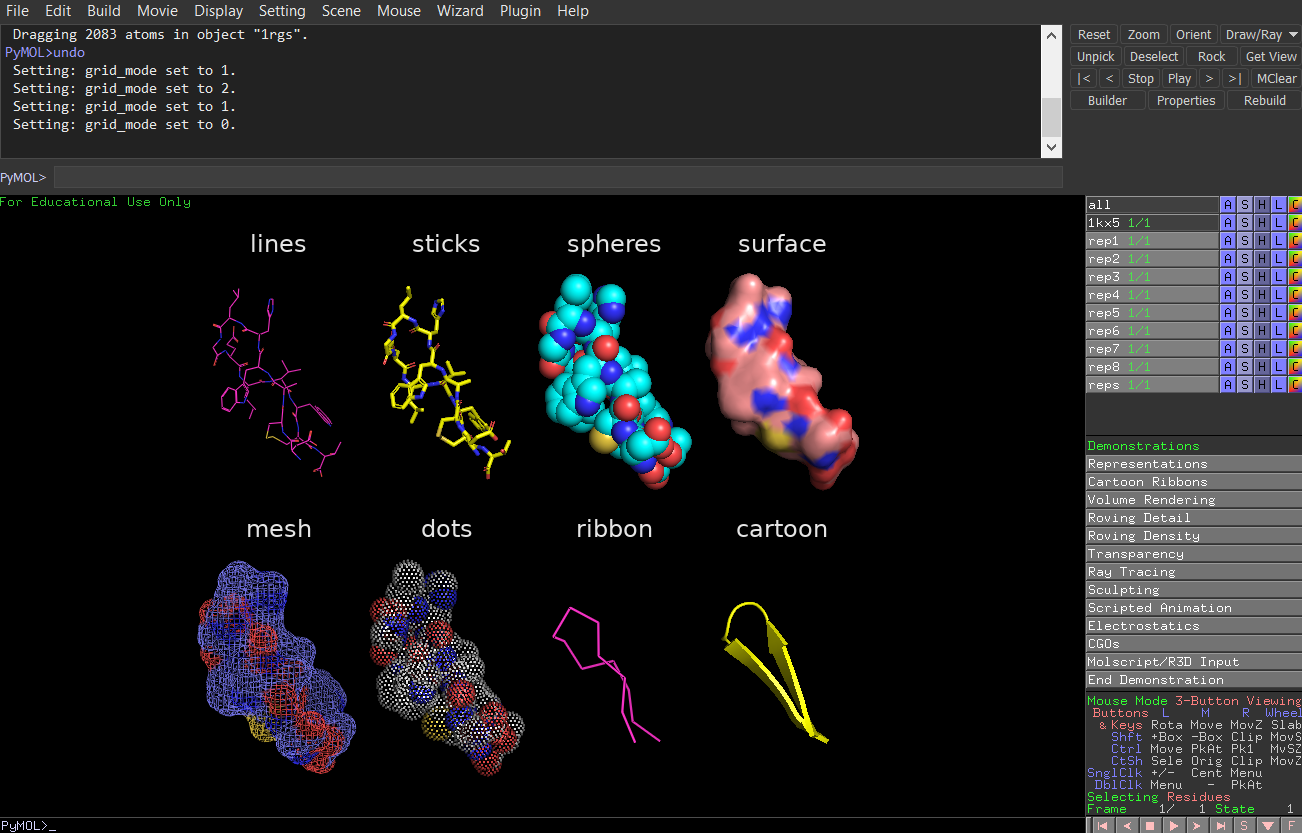
\includegraphics[width=0.8\textwidth]{workshops/pymol/imgs/representation.png}
    \caption[]{}
    \label{representation}
\end{figure}




































% \section*{Introduction} % Unnumbered section

% Lorem ipsum dolor sit amet, consectetur adipiscing elit. Praesent porttitor arcu luctus, imperdiet urna iaculis, mattis eros. Pellentesque iaculis odio vel nisl ullamcorper, nec faucibus ipsum molestie. Sed dictum nisl non aliquet porttitor. Etiam vulputate arcu dignissim, finibus sem et, viverra nisl. Aenean luctus congue massa, ut laoreet metus ornare in. Nunc fermentum nisi imperdiet lectus tincidunt vestibulum at ac elit. Nulla mattis nisl eu malesuada suscipit.

% % Math equation/formula
% \begin{equation}
% 	I = \int_{a}^{b} f(x) \; \text{d}x.
% \end{equation}

% Aliquam arcu turpis, ultrices sed luctus ac, vehicula id metus. Morbi eu feugiat velit, et tempus augue. Proin ac mattis tortor. Donec tincidunt, ante rhoncus luctus semper, arcu lorem lobortis justo, nec convallis ante quam quis lectus. Aenean tincidunt sodales massa, et hendrerit tellus mattis ac. Sed non pretium nibh. Donec cursus maximus luctus. Vivamus lobortis eros et massa porta porttitor.

% \begin{info} % Information block
% 	This is an interesting piece of information, to which the reader should pay special attention. Fusce varius orci ac magna dapibus porttitor. In tempor leo a neque bibendum sollicitudin. Nulla pretium fermentum nisi, eget sodales magna facilisis eu. Praesent aliquet nulla ut bibendum lacinia. Donec vel mauris vulputate, commodo ligula ut, egestas orci. Suspendisse commodo odio sed hendrerit lobortis. Donec finibus eros erat, vel ornare enim mattis et.
% \end{info}

% %----------------------------------------------------------------------------------------
% %	PROBLEM 1
% %----------------------------------------------------------------------------------------

% \section{Problem title} % Numbered section

% In hac habitasse platea dictumst. Curabitur mattis elit sit amet justo luctus vestibulum. In hac habitasse platea dictumst. Pellentesque lobortis justo enim, a condimentum massa tempor eu. Ut quis nulla a quam pretium eleifend nec eu nisl. Nam cursus porttitor eros, sed luctus ligula convallis quis. Nam convallis, ligula in auctor euismod, ligula mauris fringilla tellus, et egestas mauris odio eget diam. Praesent sodales in ipsum eu dictum.

% %------------------------------------------------

% \subsection{Theoretical viewpoint}

% Maecenas consectetur metus at tellus finibus condimentum. Proin arcu lectus, ultrices non tincidunt et, tincidunt ut quam. Integer luctus posuere est, non maximus ante dignissim quis. Nunc a cursus erat. Curabitur suscipit nibh in tincidunt sagittis. Nam malesuada vestibulum quam id gravida. Proin ut dapibus velit. Vestibulum eget quam quis ipsum semper convallis. Duis consectetur nibh ac diam dignissim, id condimentum enim dictum. Nam aliquet ligula eu magna pellentesque, nec sagittis leo lobortis. Aenean tincidunt dignissim egestas. Morbi efficitur risus ante, id tincidunt odio pulvinar vitae.

% Curabitur tempus hendrerit nulla. Donec faucibus lobortis nibh pharetra sagittis. Sed magna sem, posuere eget sem vitae, finibus consequat libero. Cras aliquet sagittis erat ut semper. Aenean vel enim ipsum. Fusce ut felis at eros sagittis bibendum mollis lobortis libero. Donec laoreet nisl vel risus lacinia elementum non nec lacus. Nullam luctus, nulla volutpat ultricies ultrices, quam massa placerat augue, ut fringilla urna lectus nec nibh. Vestibulum efficitur condimentum orci a semper. Pellentesque ut metus pretium lacus maximus semper. Sed tellus augue, consectetur rhoncus eleifend vel, imperdiet nec turpis. Nulla ligula ante, malesuada quis orci a, ultricies blandit elit.

% % Numbered question, with subquestions in an enumerate environment
% \begin{question}
% 	Quisque ullamcorper placerat ipsum. Cras nibh. Morbi vel justo vitae lacus tincidunt ultrices. Lorem ipsum dolor sit amet, consectetuer adipiscing elit.

% 	% Subquestions numbered with letters
% 	\begin{enumerate}[(a)]
% 		\item Do this.
% 		\item Do that.
% 		\item Do something else.
% 	\end{enumerate}
% \end{question}
	
% %------------------------------------------------

% \subsection{Algorithmic issues}

% In malesuada ullamcorper urna, sed dapibus diam sollicitudin non. Donec elit odio, accumsan ac nisl a, tempor imperdiet eros. Donec porta tortor eu risus consequat, a pharetra tortor tristique. Morbi sit amet laoreet erat. Morbi et luctus diam, quis porta ipsum. Quisque libero dolor, suscipit id facilisis eget, sodales volutpat dolor. Nullam vulputate interdum aliquam. Mauris id convallis erat, ut vehicula neque. Sed auctor nibh et elit fringilla, nec ultricies dui sollicitudin. Vestibulum vestibulum luctus metus venenatis facilisis. Suspendisse iaculis augue at vehicula ornare. Sed vel eros ut velit fermentum porttitor sed sed massa. Fusce venenatis, metus a rutrum sagittis, enim ex maximus velit, id semper nisi velit eu purus.

% \begin{center}
% 	\begin{minipage}{0.5\linewidth} % Adjust the minipage width to accomodate for the length of algorithm lines
% 		\begin{algorithm}[H]
% 			\KwIn{$(a, b)$, two floating-point numbers}  % Algorithm inputs
% 			\KwResult{$(c, d)$, such that $a+b = c + d$} % Algorithm outputs/results
% 			\medskip
% 			\If{$\vert b\vert > \vert a\vert$}{
% 				exchange $a$ and $b$ \;
% 			}
% 			$c \leftarrow a + b$ \;
% 			$z \leftarrow c - a$ \;
% 			$d \leftarrow b - z$ \;
% 			{\bf return} $(c,d)$ \;
% 			\caption{\texttt{FastTwoSum}} % Algorithm name
% 			\label{alg:fastTwoSum}   % optional label to refer to
% 		\end{algorithm}
% 	\end{minipage}
% \end{center}

% Fusce varius orci ac magna dapibus porttitor. In tempor leo a neque bibendum sollicitudin. Nulla pretium fermentum nisi, eget sodales magna facilisis eu. Praesent aliquet nulla ut bibendum lacinia. Donec vel mauris vulputate, commodo ligula ut, egestas orci. Suspendisse commodo odio sed hendrerit lobortis. Donec finibus eros erat, vel ornare enim mattis et.

% % Numbered question, with an optional title
% \begin{question}[\itshape (with optional title)]
% 	In congue risus leo, in gravida enim viverra id. Donec eros mauris, bibendum vel dui at, tempor commodo augue. In vel lobortis lacus. Nam ornare ullamcorper mauris vel molestie. Maecenas vehicula ornare turpis, vitae fringilla orci consectetur vel. Nam pulvinar justo nec neque egestas tristique. Donec ac dolor at libero congue varius sed vitae lectus. Donec et tristique nulla, sit amet scelerisque orci. Maecenas a vestibulum lectus, vitae gravida nulla. Proin eget volutpat orci. Morbi eu aliquet turpis. Vivamus molestie urna quis tempor tristique. Proin hendrerit sem nec tempor sollicitudin.
% \end{question}

% Mauris interdum porttitor fringilla. Proin tincidunt sodales leo at ornare. Donec tempus magna non mauris gravida luctus. Cras vitae arcu vitae mauris eleifend scelerisque. Nam sem sapien, vulputate nec felis eu, blandit convallis risus. Pellentesque sollicitudin venenatis tincidunt. In et ipsum libero. Nullam tempor ligula a massa convallis pellentesque.

% %----------------------------------------------------------------------------------------
% %	PROBLEM 2
% %----------------------------------------------------------------------------------------

% \section{Implementation}

% Proin lobortis efficitur dictum. Pellentesque vitae pharetra eros, quis dignissim magna. Sed tellus leo, semper non vestibulum vel, tincidunt eu mi. Aenean pretium ut velit sed facilisis. Ut placerat urna facilisis dolor suscipit vehicula. Ut ut auctor nunc. Nulla non massa eros. Proin rhoncus arcu odio, eu lobortis metus sollicitudin eu. Duis maximus ex dui, id bibendum diam dignissim id. Aliquam quis lorem lorem. Phasellus sagittis aliquet dolor, vulputate cursus dolor convallis vel. Suspendisse eu tellus feugiat, bibendum lectus quis, fermentum nunc. Nunc euismod condimentum magna nec bibendum. Curabitur elementum nibh eu sem cursus, eu aliquam leo rutrum. Sed bibendum augue sit amet pharetra ullamcorper. Aenean congue sit amet tortor vitae feugiat.

% In congue risus leo, in gravida enim viverra id. Donec eros mauris, bibendum vel dui at, tempor commodo augue. In vel lobortis lacus. Nam ornare ullamcorper mauris vel molestie. Maecenas vehicula ornare turpis, vitae fringilla orci consectetur vel. Nam pulvinar justo nec neque egestas tristique. Donec ac dolor at libero congue varius sed vitae lectus. Donec et tristique nulla, sit amet scelerisque orci. Maecenas a vestibulum lectus, vitae gravida nulla. Proin eget volutpat orci. Morbi eu aliquet turpis. Vivamus molestie urna quis tempor tristique. Proin hendrerit sem nec tempor sollicitudin.

% % File contents
% \begin{file}[hello.py]
% \begin{lstlisting}[language=Python]
% #! /usr/bin/python

% import sys
% sys.stdout.write("Hello World!\n")
% \end{lstlisting}
% \end{file}

% Fusce eleifend porttitor arcu, id accumsan elit pharetra eget. Mauris luctus velit sit amet est sodales rhoncus. Donec cursus suscipit justo, sed tristique ipsum fermentum nec. Ut tortor ex, ullamcorper varius congue in, efficitur a tellus. Vivamus ut rutrum nisi. Phasellus sit amet enim efficitur, aliquam nulla id, lacinia mauris. Quisque viverra libero ac magna maximus efficitur. Interdum et malesuada fames ac ante ipsum primis in faucibus. Vestibulum mollis eros in tellus fermentum, vitae tristique justo finibus. Sed quis vehicula nibh. Etiam nulla justo, pellentesque id sapien at, semper aliquam arcu. Integer at commodo arcu. Quisque dapibus ut lacus eget vulputate.

% % Command-line "screenshot"
% \begin{commandline}
% 	\begin{verbatim}
% 		$ chmod +x hello.py
% 		$ ./hello.py

% 		Hello World!
% 	\end{verbatim}
% \end{commandline}

% Vestibulum sodales orci a nisi interdum tristique. In dictum vehicula dui, eget bibendum purus elementum eu. Pellentesque lobortis mattis mauris, non feugiat dolor vulputate a. Cras porttitor dapibus lacus at pulvinar. Praesent eu nunc et libero porttitor malesuada tempus quis massa. Aenean cursus ipsum a velit ultricies sagittis. Sed non leo ullamcorper, suscipit massa ut, pulvinar erat. Aliquam erat volutpat. Nulla non lacus vitae mi placerat tincidunt et ac diam. Aliquam tincidunt augue sem, ut vestibulum est volutpat eget. Suspendisse potenti. Integer condimentum, risus nec maximus elementum, lacus purus porta arcu, at ultrices diam nisl eget urna. Curabitur sollicitudin diam quis sollicitudin varius. Ut porta erat ornare laoreet euismod. In tincidunt purus dui, nec egestas dui convallis non. In vestibulum ipsum in dictum scelerisque.

% % Warning text, with a custom title
% \begin{warn}[Notice:]
%   In congue risus leo, in gravida enim viverra id. Donec eros mauris, bibendum vel dui at, tempor commodo augue. In vel lobortis lacus. Nam ornare ullamcorper mauris vel molestie. Maecenas vehicula ornare turpis, vitae fringilla orci consectetur vel. Nam pulvinar justo nec neque egestas tristique. Donec ac dolor at libero congue varius sed vitae lectus. Donec et tristique nulla, sit amet scelerisque orci. Maecenas a vestibulum lectus, vitae gravida nulla. Proin eget volutpat orci. Morbi eu aliquet turpis. Vivamus molestie urna quis tempor tristique. Proin hendrerit sem nec tempor sollicitudin.
% \end{warn}

%----------------------------------------------------------------------------------------

\end{document}
